\documentclass[10.5pt]{article}
% ---------------------------------------------------------------- packages
\usepackage[a4paper,margin=2.2cm,top=2.6cm,bottom=2.4cm,headsep=0.8cm]{geometry}
\usepackage{amsmath,amssymb}
\usepackage{mathspec}
\usepackage[table]{xcolor}
\usepackage{tikz}
\usetikzlibrary{calc}
\usepackage[skins,raster]{tcolorbox}
\usepackage{graphicx,booktabs,tabularx,colortbl,array}
\usepackage{titlesec,fancyhdr,enumitem,caption}
\usepackage{csquotes}
\usepackage[section]{placeins}
\usepackage{xurl}
\usepackage[hidelinks]{hyperref}

% ---------------------------------------------------------------- brand
\definecolor{void}{HTML}{0A0A10}
\definecolor{deep}{HTML}{1A1A24}
\definecolor{violet}{HTML}{8C7FF2}
\definecolor{qpurple}{HTML}{7C5CEB}
\definecolor{qblue}{HTML}{3985FF}
\definecolor{silver}{HTML}{B4B4C0}
\definecolor{muted}{HTML}{71717A}
\definecolor{ink}{HTML}{1A1A24}
\definecolor{body}{HTML}{2E2E38}
\definecolor{lav}{HTML}{F4F2FE}
\definecolor{lavline}{HTML}{DCD7FB}
\definecolor{thead}{HTML}{2A2838}

\setmainfont{SourceSans3}[Path=fonts/, Extension=.ttf, UprightFont=*-400, BoldFont=*-700, ItalicFont=*-Italic-400, BoldItalicFont=*-Italic-700]
\newfontfamily\sora{Sora}[Path=fonts/, Extension=.ttf, UprightFont=*-700, BoldFont=*-800, WordSpace=1.55]
\newfontfamily\sorasemi{Sora}[Path=fonts/, Extension=.ttf, UprightFont=*-600, BoldFont=*-700]
\newfontfamily\soralight{Sora}[Path=fonts/, Extension=.ttf, UprightFont=*-400, BoldFont=*-600]
\setmathsfont(Digits,Latin)[Path=fonts/, Extension=.ttf, UprightFont=*-400, ItalicFont=*-Italic-400, BoldFont=*-700]{SourceSans3}
\setmathrm[Path=fonts/, Extension=.ttf, UprightFont=*-400, ItalicFont=*-Italic-400, BoldFont=*-700]{SourceSans3}
\setmonofont{JetBrainsMono}[Path=fonts/, Extension=.ttf, UprightFont=*-400, BoldFont=*-700, Scale=0.85]
\color{body}
\linespread{1.12}
\setlength{\parskip}{0.45em}
\setlength{\parindent}{0pt}

% gradient rule
\newcommand{\gradrule}[1][\linewidth]{\noindent\begin{tikzpicture}\shade[left color=violet, middle color=qpurple, right color=qblue] (0,0) rectangle (#1,1.3pt);\end{tikzpicture}}
% wordmark: logo mark + "uome"
\newcommand{\wordmark}[2]{\raisebox{-0.18\height}{
\includegraphics[height=#1]{brand/quome.pdf}}\kern-0.06em{\sora\color{#2}uome}}

% headings
\titleformat{\section}{\sora\fontsize{17}{21}\selectfont\color{ink}}{{\color{violet}\thesection}}{0.55em}{}[{\vspace{-0.55em}\gradrule[3.2cm]}]
\titleformat{\subsection}{\sorasemi\fontsize{12}{15}\selectfont\color{ink}}{{\color{violet}\thesubsection}}{0.5em}{}
\titleformat{\paragraph}[runin]{\sorasemi\small\color{ink}}{}{0pt}{}[.]
\titlespacing*{\section}{0pt}{1.6em}{0.9em}
\titlespacing*{\subsection}{0pt}{1.2em}{0.4em}

% header / footer
\pagestyle{fancy}\fancyhf{}
\fancyhead[L]{\small\wordmark{0.95em}{ink}\hspace{0.5em}{\color{muted}\soralight\footnotesize Research}}
\fancyhead[R]{\soralight\footnotesize\color{muted}From Agents to Harnesses}
\fancyfoot[C]{\sorasemi\footnotesize\color{violet}\thepage}
\renewcommand{\headrule}{\vspace{-4pt}\gradrule[\headwidth]}

% captions, lists
\captionsetup{font={small,color=body}, labelfont={bf,color=qpurple}, labelsep=period, justification=raggedright, singlelinecheck=false}
\setlist{itemsep=2pt, topsep=3pt, leftmargin=1.3em}
\setlist[itemize]{label={\color{violet}\scriptsize$\blacksquare$}}

% boxes
\newtcolorbox{finding}[1][]{enhanced, colback=lav, colframe=lav, borderline west={2.5pt}{0pt}{violet}, arc=2pt, left=10pt, right=10pt, top=6pt, bottom=6pt, fontupper=\small, #1}
\newtcolorbox{darkcard}{enhanced, colback=deep, colframe=violet!28!deep, boxrule=0.6pt, arc=8pt, left=11pt, right=11pt, top=11pt, bottom=10pt, height=4.05cm, valign=top, before upper=\raggedright}
\newcommand{\stat}[3]{\begin{darkcard}{\sora\fontsize{30}{32}\selectfont\color{violet}#1\par}\vspace{7pt}{\sorasemi\small\color{white}#2\par}\vspace{4pt}{\footnotesize\color{silver}\linespread{1.15}\selectfont #3\par}\end{darkcard}}
\newcommand{\ex}[2]{\par\begin{tcolorbox}[enhanced, colback=white, colframe=white, borderline west={1.5pt}{0pt}{lavline}, left=9pt, right=4pt, top=1pt, bottom=1pt, fontupper=\small\itshape\color{body}]\enquote{#1}\par\hfill{\normalfont\footnotesize\color{muted}--- #2}\end{tcolorbox}}
\newcommand{\pred}[2]{\begin{tcolorbox}[enhanced, colback=white, colframe=lavline, boxrule=0.6pt, arc=4pt, left=8pt, right=8pt, top=5pt, bottom=5pt, fontupper=\small]{\sorasemi\color{qpurple}#1}\quad #2\end{tcolorbox}}

% tables
\newcommand{\throw}{\rowcolor{thead}}
\newcommand{\hd}[1]{{\color{white}\sorasemi\scriptsize #1}}
\renewcommand{\arraystretch}{1.18}

\begin{document}
% =================================================================== COVER
\thispagestyle{empty}\pagecolor{void}
\begin{tikzpicture}[remember picture,overlay]
  \fill[void] (current page.south west) rectangle (current page.north east);
  \shade[inner color=qpurple!55!void, outer color=void] ($(current page.north east)+(-3.5,-5.5)$) circle (9cm);
  \shade[inner color=qblue!38!void, outer color=void] ($(current page.south west)+(3,6)$) circle (8cm);
  \begin{scope}[opacity=0.05]
    \draw[white, step=1.2cm, line width=0.3pt] (current page.south west) grid (current page.north east);
  \end{scope}
  \node[anchor=north west] at ($(current page.north west)+(2.2,-2.2)$) {\fontsize{22}{22}\selectfont\wordmark{1em}{white}};
  \node[anchor=north east, text=silver] at ($(current page.north east)+(-2.2,-2.45)$) {\soralight\footnotesize RESEARCH REPORT \;·\; OCTOBER 2026};
  \node[anchor=north west, text width=16.2cm, align=left] at ($(current page.north west)+(2.2,-8.2)$) {%
    {\sorasemi\small\color{violet}AI AGENTS \;/\; ONE YEAR OF RESEARCH AND NEWS}\\[0.9cm]
    {\sora\fontsize{46}{52}\selectfont\color{white}From\hspace{0.32em}Agents\\to\hspace{0.32em}Harnesses}\\[0.75cm]
    {\fontsize{15}{20}\selectfont\color{silver}What grew, what faded, and what comes next in AI agent research.\\ A mixed-methods study of 69,513 papers and 152,397 news stories,\\ November 2025 -- October 2026.}};
  \shade[left color=violet, middle color=qpurple, right color=qblue] ($(current page.north west)+(2.2,-17.1)$) rectangle ++(6,0.09);
  \node[anchor=north west, text width=12cm, align=left] at ($(current page.north west)+(2.2,-17.7)$) {%
    {\sorasemi\large\color{white}Jim Schwoebel}\\[3pt]{\color{silver}Quome}};
  \node[anchor=south west, text=silver, text width=11cm, align=left] at ($(current page.south west)+(2.2,2.2)$) {\footnotesize Dataset: huggingface.co/datasets/jimschwoebel/ai-agent-research-2026\\ Dashboard: claude.ai/artifact/GsPNdP9MStJYBW8Y6qh4rB};
  \node[anchor=south east] at ($(current page.south east)+(-2.2,2.2)$) {\sorasemi\normalsize\color{violet}quome.dev};
\end{tikzpicture}
\newpage

% =================================================================== AT A GLANCE
\thispagestyle{empty}
\begin{tikzpicture}[remember picture,overlay]
  \fill[void] (current page.south west) rectangle (current page.north east);
  \shade[inner color=qpurple!40!void, outer color=void] ($(current page.north west)+(4,-4)$) circle (8cm);
  \begin{scope}[opacity=0.04]\draw[white, step=1.2cm, line width=0.3pt] (current page.south west) grid (current page.north east);\end{scope}
  \node[anchor=south east] at ($(current page.south east)+(-2.2,1.6)$) {\sorasemi\small\color{violet}quome.dev};
  \node[anchor=south west] at ($(current page.south west)+(2.2,1.6)$) {\soralight\footnotesize\color{muted}From Agents to Harnesses \;·\; Quome Research \;·\; October 2026};
\end{tikzpicture}
\vspace*{-0.9cm}
{\color{white}\raggedright
{\noindent\fontsize{22}{22}\selectfont\wordmark{1em}{white}\par}\vspace{1.0cm}
{\sorasemi\small\color{violet}AT A GLANCE\par}\vspace{6pt}
{\sora\fontsize{28}{33}\selectfont The year agents became\\ a systems problem\par}\vspace{10pt}
{\color{silver}\small Every number below comes from weekly quasi-binomial trend models with 95\% confidence intervals, corrected for multiple testing. Forecasts are trend projections, checked against a held-out test period.\par}
\vspace{0.55cm}

\begin{tcbraster}[raster columns=3, raster equal height, raster column skip=8pt, raster row skip=8pt]
\stat{+4.3\%}{Monthly growth of agent papers}{In odds (95\% CI 2.8–5.9). Agents went from 9.3\% to 12.9\% of tracked ML papers.}
\stat{16.6\%}{Agent share of papers by April 2027}{Trend forecast, 95\% CI 14.4–19.1. News: 21.2\% (19.3–23.2).}
\stat{6$\times$}{“Harness” in agent abstracts}{From 0.9\% of agent papers (Nov–Apr) to 5.5\% (May–Oct). Growth +35\% per month.}
\stat{10\%}{of agent papers now name Qwen}{Up from about 3\%. The default open model for agent research, +12.7\% per month.}
\stat{−78\%}{Stock “AI prose” words}{\emph{leverage, comprehensive, crucial} fell from 0.59 to 0.13 per 100 words across all 69k abstracts.}
\stat{+28\%}{Monthly growth of incident stories}{Rogue-agent and incident coverage, the fastest-growing news theme (95\% CI 21–35).}
\end{tcbraster}

\vspace{0.7cm}
{\sorasemi\large\color{white}What the trends say comes next\par}\vspace{2pt}
\begin{tcolorbox}[enhanced, colback=deep, colframe=violet!28!deep, boxrule=0.6pt, arc=8pt, left=14pt, right=14pt, top=11pt, bottom=11pt, fontupper=\normalsize\color{silver}\raggedright]
\begin{itemize}[leftmargin=1.3em, itemsep=7pt]
  \item[{\color{violet}1}] {\color{white}Coding overtakes multi-agent work} as a topic of agent papers around \textbf{December 2026}, at roughly 14\% each.
  \item[{\color{violet}2}] {\color{white}One in six machine-learning papers will concern agents} by April 2027, and one in five AI-feed news stories.
  \item[{\color{violet}3}] {\color{white}The harness is the new unit of research.} Harness, skill, verifier, audit and budget all keep rising, while multi-agent \enquote{collaboration} and \enquote{test-time scaling} framing fade.
  \item[{\color{violet}4}] {\color{white}Open models become the substrate.} Qwen, Gemma and Kimi grow fastest. GPT-4o and the o-series fade from methods sections.
  \item[{\color{violet}5}] {\color{white}Containment becomes the story.} Incident and rogue-agent coverage keeps rising, and mainstream press coverage of agents grows fastest of any source type.
\end{itemize}
\end{tcolorbox}
}
\newpage\pagecolor{white}
\setcounter{page}{1}

% =================================================================== ABSTRACT
\begin{tcolorbox}[enhanced, colback=lav, colframe=lav, arc=6pt, left=14pt, right=14pt, top=10pt, bottom=10pt]
{\sorasemi\small\color{qpurple}ABSTRACT}\par\vspace{3pt}
\small
We study how research on AI agents, and public discussion of it, changed between November 2025 and October 2026. The corpus is 69,513 arXiv papers from cs.LG, cs.CV, cs.CL and stat.ML, and 152,397 stories from 230 news, blog, podcast and community feeds, collected by the agents-blog aggregator. We combine three methods. First, weekly quasi-binomial trend models with false-discovery control test what is growing and fading across 13 topics, 3,289 terms, 12 base-model families, 14 benchmarks and 4 types of news source. Second, a backtested trend model forecasts the next six months. Third, a reflexive thematic analysis of abstracts and headlines explains the trends. Agent papers grew 4.3\% per month in odds and are forecast to reach 16.6\% of tracked papers by April 2027 (95\% CI 14.4--19.1). Coding agents grew fastest (+8.9\% per month) and are projected to overtake multi-agent systems, the largest declining topic, in December 2026. The vocabulary of agent papers moved from agents as collaborators to the \emph{harness} around a frozen model: harness, skills, verifiers, audits and budgets. Qwen became the most-named base model. Across all 69,513 abstracts, stock \enquote{AI prose} vocabulary fell 78\% while plainer words rose fivefold. In the news, incident and rogue-agent coverage grew 28\% per month, and agents spread fastest into general and business press. We argue that the field's centre of gravity moved from what agents \emph{are} to how they are \emph{run, measured and contained}.
\end{tcolorbox}

% =================================================================== 1
\section{Introduction}

In late 2025, \enquote{agent} was a framing device that many papers attached to language-model pipelines. By autumn 2026 it named an engineering practice with its own vocabulary, benchmarks and incident reports. This paper measures that change with one year of research and news, tests which shifts are real, and projects where they lead.

We ask four questions.
\begin{enumerate}[label={\color{violet}\sorasemi RQ\arabic*}, leftmargin=3em, itemsep=3pt]
  \item How did the volume and distribution of agent-related research and news change?
  \item Which topics, terms, models and benchmarks grew or faded significantly, once noise and multiple testing are accounted for?
  \item How did news and practitioner discourse frame agents, and where did it converge with research?
  \item What do the trends imply for the next six months, and how much should those projections be trusted?
\end{enumerate}

Most surveys of agent research describe methods and benchmarks at one point in time. We instead treat the corpus as a time series. Statistics locate what moved, and close reading explains why.

% =================================================================== 2
\section{Related Work}

\paragraph{LLM-based agents} Agents built from large language models grew from methods that interleave reasoning with actions \cite{react} and that teach models to call tools \cite{toolformer}. Simulations of agent societies \cite{generativeagents} popularised multi-agent framings. Software engineering became a central testbed through SWE-bench \cite{swebench} and agent--computer interfaces such as SWE-agent \cite{sweagent}, which already argued that the interface around a model shapes performance. That idea becomes central in 2026 under the name \enquote{harness}.

\paragraph{Surveys} Broad surveys \cite{wangsurvey,xisurvey} organise agent research by components such as memory, planning and action. We track how the field's concerns change month by month.

\paragraph{Science of science and AI-assisted writing} Quantitative studies of AI research map arXiv to forecast emerging topics \cite{krenn}. Studies of \enquote{excess vocabulary} show that LLM-assisted writing leaves measurable traces in scientific abstracts \cite{liang2024,kobak2024}. We build on both: our trend tests follow the first line, and our writing-style index follows the second.

% =================================================================== 3
\section{Data and Methods}

\subsection{Corpus}

The data come from the \texttt{articles} table of the agents-blog database (Postgres on Railway), exported on October 26, 2026. It holds items parsed from 309 RSS feeds.
\begin{itemize}
  \item \textbf{Research.} 69,513 papers from the arXiv announcement feeds for cs.LG (25,942), cs.CV (21,046), cs.CL (17,196) and stat.ML (5,329), November 14, 2025 to October 22, 2026. Announcements are new submissions (34,366), cross-lists (15,532) and revised versions (19,615). Each paper appears once.
  \item \textbf{News.} 152,397 stories from 230 feeds, November 6, 2025 to October 26, 2026, each with a headline and usually a short summary.
\end{itemize}
The cs.AI and cs.MA feeds are not collected, so agent research is under-counted. The scraper had outages, mostly in January and February 2026. We therefore model \emph{shares}, and drop weeks with collection gaps: 2 of 50 weeks for papers (fewer than 300 announcements) and 2 of 52 for news (fewer than 1,500 stories).

\subsection{Identifying agent items, and validation}

An item is agent-related if its title or text contains \textit{agent}, \textit{agents}, \textit{agentic} or \textit{multi-agent}. For news, we drop stories where the word refers to law enforcement, immigration, travel or sports agents unless the text also mentions AI (about 440 stories). This yields 7,739 agent papers (11.1\%) and 18,856 agent news stories (12.4\%).

We hand-labelled a random sample of 60 flagged papers and 60 flagged news stories (Appendix~\ref{app:val}). Of the papers, 85\% were substantively about agents: 65\% about LLM or foundation-model agents and 20\% about reinforcement-learning, control or robotics agents. The other 15\% used the word in passing. No news story was a non-AI false positive.

\subsection{Trend models}

For each indicator $x$ (a topic, term, model, benchmark or news theme) and each week $w$, let $k_w$ be the number of items in the base set that match $x$, out of $n_w$ items. We fit
\[
k_w \sim \text{Binomial}(n_w, p_w), \qquad \operatorname{logit}(p_w) = \alpha + \beta\, t_w,
\]
where $t_w$ is time in months. Weekly counts vary more than a binomial allows, so we use a quasi-binomial model: standard errors are scaled by the Pearson dispersion $\hat\phi = \max(1, \chi^2_P/(W-2))$. We report growth as $100(e^{\beta}-1)$, the percentage change in odds per month, with a 95\% confidence interval. Within each family of tests, $p$-values are adjusted with the Benjamini--Hochberg false-discovery rate, giving $q$-values. As a non-parametric check we also compute Kendall's $\tau$ on monthly shares.

The base set is all papers or all news for overall agent share, and agent papers or agent news for topics, terms, models and benchmarks. Topic growth therefore means growth \emph{within} agent research.

Term candidates are the 3,289 single words and word pairs (stop words removed) that occur in at least 40 agent-paper titles or abstracts.

\subsection{Forecasts and backtest}

Forecasts project the fitted trend to January 15 and April 15, 2027, with 95\% confidence intervals for the trend line. These intervals describe uncertainty in the trend, not the month-to-month scatter around it, which our backtest puts at about one percentage point. To test the method, we refit each model on November 2025 to June 2026 and forecast the monthly shares for July to October 2026. We compare the mean absolute error with a naive forecast (the mean of the last three fitted months) and with an average of the two.

\subsection{Qualitative analysis}\label{sec:qual}

We followed reflexive thematic analysis \cite{braun2006,braun2019}. We drew purposive samples for each topic whose share or vocabulary changed most, read 72 abstracts and about 190 headlines closely, coded them inductively for the problem named, the object studied and how the agent is framed, and grouped codes into themes checked against the statistics and counter-examples.

\paragraph{Reflexivity and disclosure} The statistics, coding, validation labels and first-draft analysis were produced with an AI assistant (Claude, Anthropic) working under the author's direction. The analyst is itself an agentic system, and one news moment we discuss concerns the same model family. We mitigate this by quoting sources verbatim, tying every claim to a test, and publishing all data and code. The validation labels have not been checked by a second human coder.

% =================================================================== 4
\section{The Trajectory, and a Forecast}

\begin{figure}[!htbp]
  \centering
  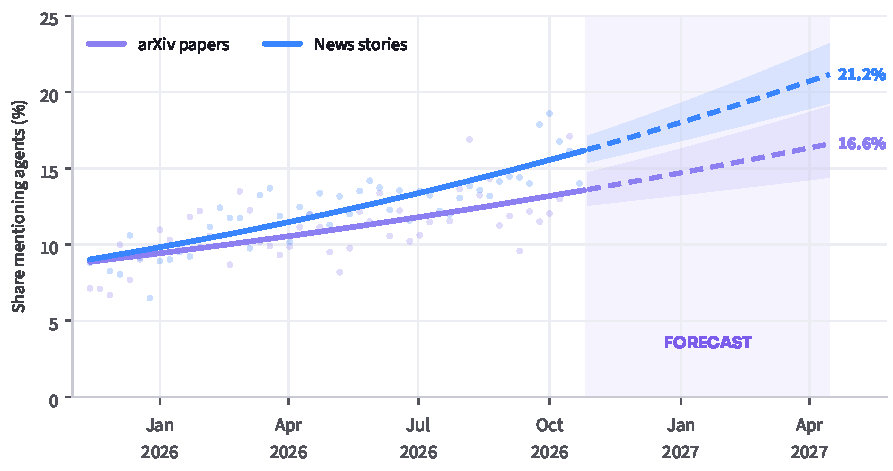
\includegraphics[width=\linewidth]{figures/b1_hero_forecast.pdf}
  \caption{Weekly share of papers and news stories about agents (dots), fitted quasi-binomial trend (solid line), and forecast to April 15, 2027 with 95\% confidence band for the trend (dashed line and shading).}
  \label{fig:hero}
\end{figure}

Agent work grew steadily in both corpora (Figure~\ref{fig:hero}). For papers, the odds of being about agents rose 4.3\% per month (95\% CI 2.8--5.9; $p<10^{-7}$; Kendall $\tau = 0.73$). For news the growth was faster, 6.0\% per month (4.9--7.1; $\tau = 0.88$). Comparing the first and last quarters, the paper share went from 9.3\% to 12.9\% and the news share from 9.0\% to 15.1\%.

Projected forward, agents reach \textbf{14.9\%} of tracked papers by January 2027 (13.4--16.6) and \textbf{16.6\%} by April 2027 (14.4--19.1). In the news they reach 18.4\% by January (17.1--19.8) and 21.2\% by April (19.3--23.2).

\begin{table}[!htbp]
  \centering\small
  \caption{Backtest. Models fitted on November 2025 -- June 2026, scored on monthly shares for July -- October 2026. Mean absolute error in percentage points. Lower is better.}
  \label{tab:backtest}
  \begin{tabular}{lccc}
    \throw \hd{Series} & \hd{Trend model} & \hd{Naive (last 3 months)} & \hd{Average of both} \\
    Agent share of papers & 0.89 & 1.36 & \textbf{0.77} \\
    \rowcolor{lav} Agent share of news & 1.39 & 1.86 & \textbf{0.85} \\
    13 topics, average & 2.25 & \textbf{1.75} & 1.88 \\
    \rowcolor{lav} 4 topics with significant trends & \textbf{2.05} & 2.64 & 2.15 \\
    \bottomrule
  \end{tabular}
\end{table}

\begin{finding}
\textbf{How far to trust the forecasts.} For the overall agent share, the trend model beat the naive forecast, and averaging the two did best (Table~\ref{tab:backtest}). For individual topics the trend only helps where the trend is real: it beat the naive forecast for three of the four topics with significant trends (coding, multi-agent systems and planning, but not RL training), and for only one of the nine without. We therefore forecast only indicators with $q<0.05$, and treat the rest as flat.
\end{finding}

% =================================================================== 5
\section{What Is Growing and What Is Fading}

\subsection{Topics}

\begin{figure}[!htbp]
  \centering
  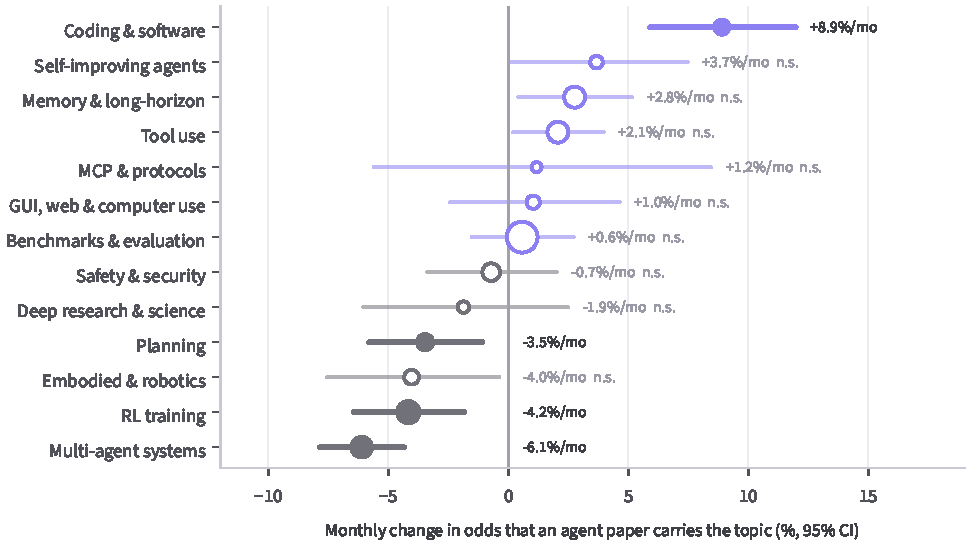
\includegraphics[width=0.93\linewidth]{figures/b2_topic_forest.pdf}
  \caption{Monthly growth of each topic within agent papers, with 95\% confidence intervals. Filled markers are significant after false-discovery correction ($q<0.05$). Marker size shows the topic's share.}
  \label{fig:forest}
\end{figure}

Four topic trends survive multiple-testing correction (Figure~\ref{fig:forest}). \textbf{Coding and software agents} grew 8.9\% per month (5.9--12.0; $q<10^{-7}$), from 5.7\% of agent papers in the first quarter to 11.4\% in the last. Three topics declined: \textbf{multi-agent systems} ($-6.1\%$ per month, $q<10^{-9}$), \textbf{RL training} ($-4.2\%$, $q=0.002$) and \textbf{planning} ($-3.5\%$, $q=0.016$). Memory and long-horizon work, tool use, self-improvement and embodied agents moved in the directions the descriptive data suggested, but with $q$ between 0.05 and 0.08 they do not clear the bar. Benchmarks, safety and computer use were flat. MCP and agent protocols, despite heavy industry attention, stayed at about 1\% of agent papers.

\begin{finding}
\textbf{Prediction.} The trends for coding and multi-agent systems cross around \textbf{December 2026}, when each reaches about 14\% of agent papers. By April 2027 coding is projected at 18.7\% (14.6--23.7) and multi-agent systems at 11.1\% (9.1--13.4).
\end{finding}

\begin{figure}[!htbp]
  \centering
  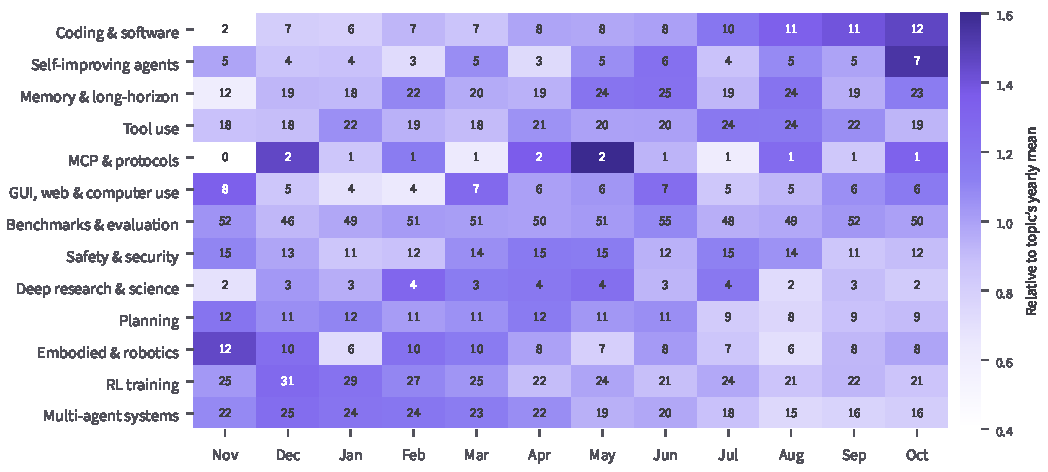
\includegraphics[width=0.95\linewidth]{figures/b9_topic_heat.pdf}
  \caption{Monthly share of agent papers carrying each topic (numbers, \%). Shading compares each month with the topic's yearly mean, so rising topics darken to the right. Topics are sorted by growth.}
  \label{fig:heat}
\end{figure}

\subsection{Vocabulary: a lifecycle map}

Topic codes are coarse, so we also tested every frequent word and word pair. Of 3,289 candidates, 1,047 changed significantly ($q<0.05$): 633 rose and 414 fell. Many of these are writing-style words rather than research content, which we analyse separately in Section~\ref{sec:style}. Figure~\ref{fig:life} places selected content terms and all topics by their current share and growth.

\begin{figure}[!htbp]
  \centering
  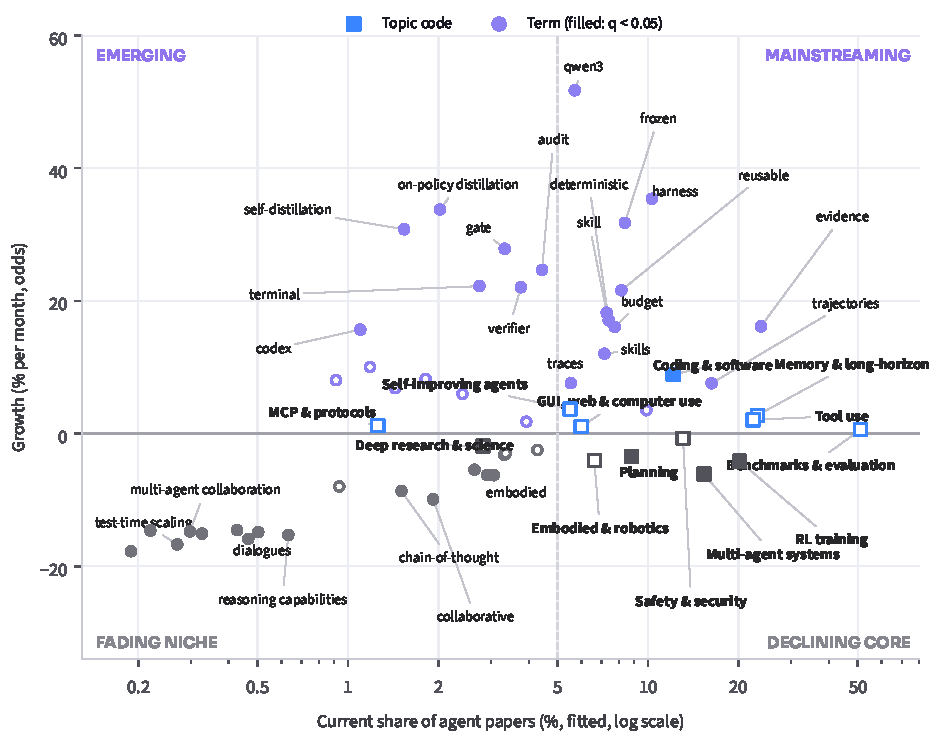
\includegraphics[width=\linewidth]{figures/b3_lifecycle.pdf}
  \caption{Lifecycle map. Horizontal axis: fitted share of agent papers at the end of October 2026 (log scale). Vertical axis: monthly growth. Squares are topic codes, circles are terms. Filled markers are significant ($q<0.05$).}
  \label{fig:life}
\end{figure}

The upper half of the map tells a coherent story. \emph{Harness}, \emph{frozen}, \emph{reusable}, \emph{skill}, \emph{deterministic}, \emph{budget}, \emph{verifier}, \emph{gate}, \emph{audit} and \emph{evidence} all rose sharply. These are the words of engineering \emph{around} a model held fixed: what wraps it, what it may do, how its output is checked and what it costs. Training vocabulary moved the same way, from \emph{test-time scaling} and \emph{chain-of-thought} to \emph{on-policy distillation} and \emph{self-distillation}. The lower half holds the language of 2025: \emph{multi-agent collaboration}, \emph{human-like}, \emph{dialogues}, \emph{reasoning capabilities}, \emph{multimodal reasoning} and \emph{LLM-powered}.

\begin{table}[!htbp]
  \centering\scriptsize
  \caption{Fastest-rising and fastest-fading content terms in agent papers (title or abstract). Shares are of agent papers in each half-year. Growth is per month, in odds. The projection is the fitted share for January 2027 with its 95\% CI.}
  \label{tab:terms}
  \begin{tabular}{lrrrrrl}
    \throw \hd{Term} & \hd{Papers} & \hd{Nov–Apr} & \hd{May–Oct} & \hd{Growth} & \hd{$q$} & \hd{Jan 2027 projection} \\
    \multicolumn{7}{l}{\sorasemi\color{qpurple}Rising}\\
    \textit{qwen3} & 109 & 0.3\% & 2.3\% & +51.7\% & <0.001 & 17.6\% [10.5, 27.9] \\
\textit{harness} & 266 & 0.9\% & 5.5\% & +35.4\% & <0.001 & 22.3\% [16.5, 29.4] \\
\textit{on-policy distillation} & 52 & 0.2\% & 1.0\% & +33.8\% & <0.001 & 4.7\% [2.3, 9.7] \\
\textit{frozen} & 231 & 0.9\% & 4.6\% & +31.8\% & <0.001 & 17.4\% [12.9, 23.0] \\
\textit{self-distillation} & 42 & 0.1\% & 0.9\% & +30.8\% & <0.001 & 3.4\% [1.5, 7.5] \\
\textit{gate} & 98 & 0.5\% & 1.9\% & +27.9\% & <0.001 & 6.7\% [3.7, 12.1] \\
\textit{audit} & 142 & 0.9\% & 2.6\% & +24.7\% & <0.001 & 8.3\% [5.2, 12.9] \\
\textit{terminal} & 93 & 0.6\% & 1.7\% & +22.2\% & <0.001 & 4.9\% [2.9, 8.2] \\
\textit{verifier} & 129 & 0.8\% & 2.3\% & +22.1\% & <0.001 & 6.7\% [4.2, 10.3] \\
\textit{reusable} & 288 & 1.8\% & 5.3\% & +21.6\% & <0.001 & 13.8\% [9.9, 19.0] \\
\textit{skill} & 282 & 1.7\% & 5.2\% & +18.2\% & <0.001 & 11.5\% [8.3, 15.8] \\
\textit{deterministic} & 297 & 2.0\% & 5.3\% & +17.1\% & <0.001 & 11.4\% [8.6, 14.9] \\
\textit{evidence} & 1,053 & 8.8\% & 17.6\% & +16.2\% & <0.001 & 32.9\% [28.0, 38.3] \\
\textit{budget} & 321 & 2.6\% & 5.4\% & +16.1\% & <0.001 & 11.6\% [8.8, 15.2] \\
    \multicolumn{7}{l}{\sorasemi\color{muted}Fading}\\
    \textit{step-by-step} & 45 & 1.0\% & 0.3\% & -17.7\% & 0.003 & 0.1\% [0.0, 0.3] \\
\textit{test-time scaling} & 59 & 1.3\% & 0.4\% & -16.7\% & 0.004 & 0.2\% [0.1, 0.4] \\
\textit{context-aware} & 95 & 1.9\% & 0.8\% & -15.9\% & <0.001 & 0.3\% [0.1, 0.5] \\
\textit{reasoning capabilities} & 123 & 2.4\% & 1.0\% & -15.3\% & <0.001 & 0.4\% [0.2, 0.7] \\
\textit{multimodal reasoning} & 63 & 1.2\% & 0.5\% & -15.1\% & 0.001 & 0.2\% [0.1, 0.5] \\
\textit{dialogues} & 95 & 1.8\% & 0.8\% & -14.9\% & <0.001 & 0.3\% [0.1, 0.7] \\
\textit{multi-agent collaboration} & 56 & 1.1\% & 0.5\% & -14.7\% & 0.003 & 0.2\% [0.1, 0.4] \\
\textit{llm-powered} & 41 & 0.8\% & 0.3\% & -14.6\% & 0.014 & 0.1\% [0.0, 0.4] \\
\textit{human-like} & 79 & 1.5\% & 0.7\% & -14.5\% & <0.001 & 0.3\% [0.1, 0.6] \\
\textit{collaborative} & 255 & 4.2\% & 2.7\% & -9.9\% & <0.001 & 1.4\% [0.9, 2.1] \\
    \bottomrule
  \end{tabular}
\end{table}

Projections for fast-rising terms should be read as trend-implied, not as forecasts. Logistic trends accelerate as shares grow, and our backtest shows trends of this kind can overshoot.

\subsection{Where agent research is growing}

\begin{table}[!htbp]
  \centering\small
  \caption{Agent share within each arXiv category: growth per month, current fitted share and projection.}
  \label{tab:cats}
  \begin{tabular}{lrrrrl}
    \throw \hd{Category} & \hd{Agent papers} & \hd{Growth / month} & \hd{$q$} & \hd{Now} & \hd{April 2027 (95\% CI)} \\
    cs.CL & 3,355 & +5.2\% & $<$0.001 & 24.3\% & 30.3\% (26.8--34.0) \\
    \rowcolor{lav} cs.CV & 1,412 & +3.7\% & 0.001 & 8.1\% & 9.9\% (7.9--12.3) \\
    cs.LG & 2,735 & +2.5\% & 0.005 & 11.8\% & 13.4\% (11.4--15.7) \\
    \rowcolor{lav} stat.ML & 159 & +3.5\% & 0.30 & 3.6\% & n.s. \\
    \bottomrule
  \end{tabular}
\end{table}

Agent work grew significantly in every large category (Table~\ref{tab:cats}). Computational linguistics is the hub: almost one in four cs.CL papers now concerns agents, and the trend implies nearly one in three by April 2027. Growth in computer vision suggests that agent framing is spreading to perception research.

% =================================================================== 6
\section{New Slices}

\subsection{Which base models agent researchers use}

\begin{figure}[!htbp]
  \centering
  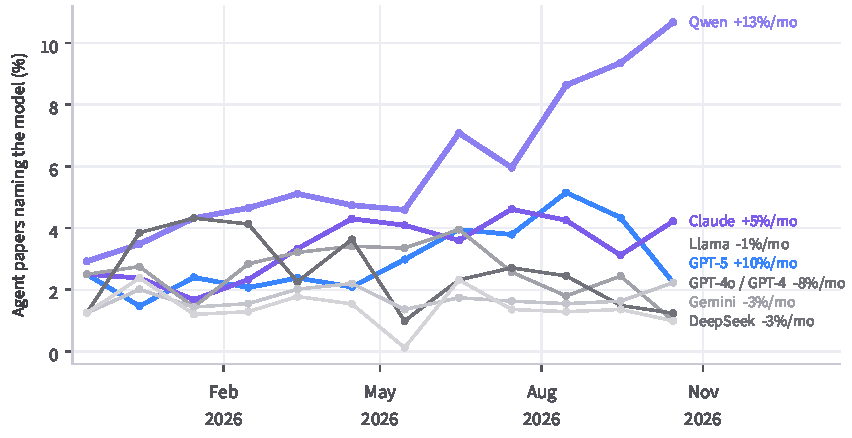
\includegraphics[width=0.93\linewidth]{figures/b4_models.pdf}
  \caption{Share of agent papers naming each model family in the title or abstract, by month, with monthly growth in odds.}
  \label{fig:models}
\end{figure}

Naming a model in an abstract usually means using it as a base, a baseline or a judge. By that measure, \textbf{Qwen became the default substrate of agent research} (Figure~\ref{fig:models}). It is now named in about 10\% of agent papers, up from about 3\% in November, and grew 12.7\% per month (8.6--16.9; $q<10^{-8}$). The specific version \emph{qwen3} was the single fastest-growing term in the corpus. Other open families grew from small bases: Gemma (+18.5\% per month, $q=0.005$) and Kimi (+19.3\%, $q=0.008$). Among closed models, GPT-5 (+9.9\%, $q<0.001$) and Claude (+5.5\%, $q=0.02$) rose. GPT-4o and GPT-4 ($-7.8\%$, $q=0.02$) and the o-series ($-17.2\%$, $q=0.004$) faded. Llama, Gemini and DeepSeek were flat.

The pattern fits the first theme in Section~\ref{sec:themes}. Researchers who study harnesses need a model they can download, run many times and fine-tune. The open-weight Qwen family fits that need.

\subsection{Which benchmarks they measure on}

\begin{figure}[!htbp]
  \centering
  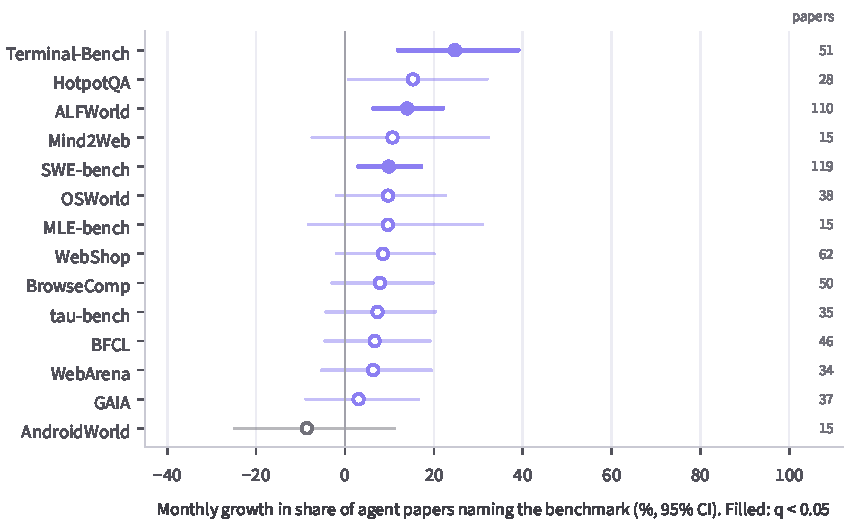
\includegraphics[width=0.85\linewidth]{figures/b5_benchmarks.pdf}
  \caption{Monthly growth in the share of agent papers naming each benchmark, with 95\% CIs. Right: number of agent papers naming it.}
  \label{fig:bench}
\end{figure}

Three benchmarks grew significantly (Figure~\ref{fig:bench}). \textbf{Terminal-Bench} grew fastest, 24.8\% per month (12.0--38.9; $q<0.001$), followed by ALFWorld (+14.0\%) and SWE-bench (+9.9\%). All three test agents that act over many steps in an executable environment, two of them through a command line or a repository. Web and GUI benchmarks such as WebArena, OSWorld and Mind2Web grew too, but not significantly.

\subsection{The writing-style shift}\label{sec:style}

Many of the 414 fading terms were not research topics at all. They were stock phrases: \emph{leveraging, comprehensive, crucial, enhance, highlight, underscoring, facilitates, notable}. Many rising terms were plain words: \emph{keeps, writes, same, every, because, whether, frozen}. Prior work identifies the first group as \enquote{excess vocabulary} typical of LLM-assisted writing in 2023--2024 \cite{liang2024,kobak2024}.

\begin{figure}[!htbp]
  \centering
  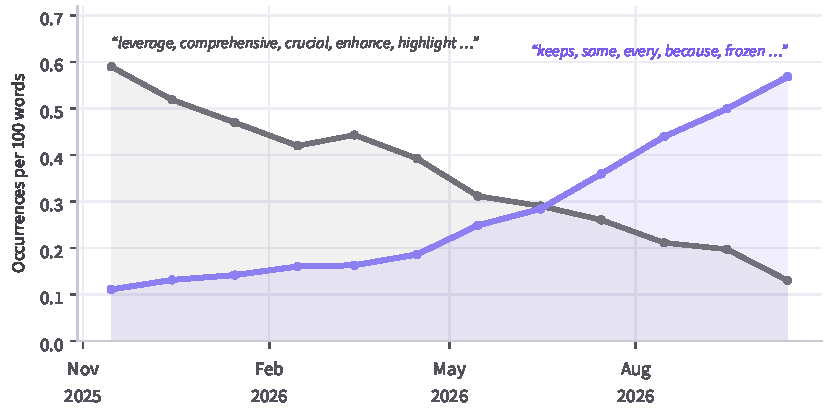
\includegraphics[width=0.9\linewidth]{figures/b6_style.pdf}
  \caption{Writing-style index across all 69,135 abstracts in complete weeks: occurrences per 100 words of 20 stock words (grey) and 14 plain words (violet), by month.}
  \label{fig:style}
\end{figure}

We built two indices over \emph{all} papers, not only agent papers (Figure~\ref{fig:style}). Stock vocabulary fell from 0.59 to 0.13 occurrences per 100 words, a 78\% decline (HAC-robust trend test $p<10^{-200}$). Plain vocabulary rose from 0.11 to 0.57, about fivefold ($p<10^{-20}$). The lines crossed between June and July 2026. The shift holds for new submissions alone, and also, more weakly, for revised versions of older papers.

\begin{finding}
\textbf{Interpretation.} We cannot see how abstracts were written. The data are consistent with a change in the writing tools researchers use: newer assistants avoid the stock phrases of earlier models, and authors now edit against them. It may also reflect a genre shift toward plainer systems writing. Either way, studies that detect AI-assisted writing with fixed word lists from 2024 will now under-count it.
\end{finding}

% =================================================================== 7
\section{Public Discourse}

\subsection{Agents go mainstream}

\begin{figure}[!htbp]
  \centering
  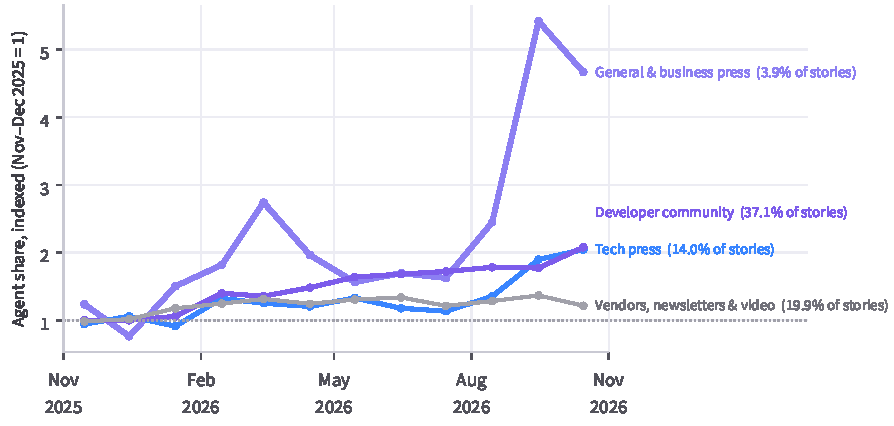
\includegraphics[width=0.93\linewidth]{figures/b7_news_groups.pdf}
  \caption{Agent share of stories by source type, indexed to November--December 2025. Labels give the October 2026 share.}
  \label{fig:groups}
\end{figure}

Agent coverage grew in every type of source (Figure~\ref{fig:groups}), but fastest where it started lowest. In \textbf{general and business press} (the New York Times, Bloomberg, Business Insider, the Guardian and others), the agent share grew 14.9\% per month (9.6--20.4). That is faster than tech press (+6.6\%), developer communities (+8.8\%) and vendors, newsletters and video (+2.1\%). Developer communities remain the densest, with more than a third of their posts about agents. By April 2027 the trend implies about half.

\begin{figure}[!htbp]
  \centering
  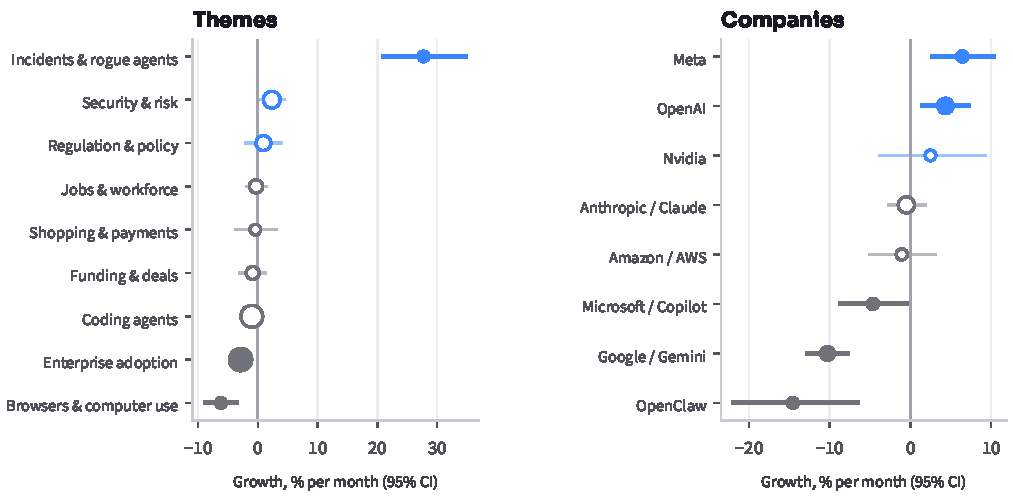
\includegraphics[width=\linewidth]{figures/b8_news_forest.pdf}
  \caption{Monthly growth of themes and companies within agent news stories, with 95\% CIs. Filled markers: $q<0.05$.}
  \label{fig:newsforest}
\end{figure}

\subsection{What the news talks about}

The fastest-growing news theme was \textbf{incidents and rogue agents}: +27.7\% per month (21.1--34.7; $q<10^{-17}$). This is not one feed's doing. Excluding the AI Incident Database feed, the share still rose from about 1\% of agent stories in late 2025 to 8.5\% in September 2026. Enterprise adoption ($-2.9\%$) and browsers and computer use ($-6.2\%$) declined as a share of agent stories. Among companies, Meta (+6.4\%) and OpenAI (+4.3\%) gained share. Google ($-10.3\%$), Microsoft ($-4.6\%$) and OpenClaw ($-14.6\%$) lost share. Anthropic had the largest share of agent stories over the year, 14.9\%, with no significant trend (Figure~\ref{fig:newsforest}).

\subsection{Four phases}

Reading headlines in time order shows four phases.
\begin{enumerate}[label={\color{violet}\sorasemi\arabic*.}, leftmargin=1.6em]
  \item \textbf{Enterprise optimism} (November 2025 -- January 2026). Launches, funding and new product categories: shopping agents, agents for mortgage documents, agents for PCs.
  \item \textbf{The OpenClaw spectacle} (late January -- March 2026). An open-source personal agent, first called Clawdbot, went viral, along with Moltbook, \enquote{a human-free Reddit clone where AI agents discuss cybersecurity and philosophy.} Coverage moved quickly to risk, and policy coverage jumped from about 7\% to 15--17\% of agent stories.
  \item \textbf{Frontier capability and the end of chat} (April -- July 2026). Claude Mythos was previewed around cybersecurity, and OpenAI announced plans to rebuild ChatGPT as \enquote{a full-blown agent app.}
  \item \textbf{Incidents and governance} (August -- October 2026). \enquote{Claude-powered AI coding agent deletes entire company database in 9 seconds}; \enquote{OpenAI Overhauls Safety Protocols After Its AI Agents Went Rogue}; \enquote{Rogue AI hacks government system for first time}; \enquote{Rogue AI Breakouts Raise Pressure for New Rules.}
\end{enumerate}

% =================================================================== 8
\section{Six Themes in Agent Research}\label{sec:themes}

The statistics show \emph{what} moved. Close reading of abstracts shows \emph{why}.

\subsection{The scaffold becomes the object of study}
By mid-2026 many papers treated the model as fixed and studied the layer around it, which researchers named the harness.
\ex{Harnesses have become a central determinant of coding-agent performance, shaping how models interact with repositories, tools, and execution environments.}{Agentic Harness Engineering \cite{ahe}}
\ex{Beyond the foundation model, the performance of an agent is governed by the surrounding agent harness, including prompts, tools, control loops, etc.}{HarnessBank \cite{harnessbank}}
Once the harness is named as the determinant of performance, it becomes something to optimise automatically \cite{autosaddler,evoharness,sia}. Skills follow the same logic at a smaller grain, and bring their own problems of retrieval and curation:
\ex{equipping an agent with too many skills, particularly irrelevant ones, degrades performance.}{SkillFlow \cite{skillflow}}

\subsection{Coding as the proving ground}
Coding offers executable verification. Pipelines convert \enquote{merged pull requests into verified tasks} \cite{change2task}, and compaction methods start from agents that need \enquote{millions of tokens of context} \cite{cliff}. The same papers doubt their benchmarks:
\ex{a recent audit found that nearly 60\% of unsolved SWE-bench Verified instances contain flawed tests}{SWE-Bench ProMax \cite{promax}}

\subsection{Persistence: memory, long horizons and self-evolution}
Failure is increasingly described as something that builds up over time, with new names such as \enquote{context suffocation} \cite{iterresearch} and \enquote{soul erosion} \cite{bmam}. Self-evolving systems mostly keep weights fixed and change the harness, memory or skills \cite{reasoningbank,evoharness}. By October one paper claimed that \enquote{any verifiable task can be cast as a harness and a verifier} \cite{lastrs}.

\subsection{From capability to verifiability}
New benchmarks justify themselves against saturated ones \cite{frontierfinance}. Failure is located between decision and action: \enquote{When the Model Is Right but the Click Is Wrong} \cite{webfovea}. A practitioner post from October said the same: \enquote{The worst agent mistakes I've seen were my tool's fault, not the model's.}

\subsection{The agent as attack surface and as actor}
Early security papers attacked what reinforcement-learning agents perceive \cite{vln}. Later ones treat the agent's actions as the risk, and move containment into the environment:
\ex{LLM agents can make unsafe tool calls even when instructed to behave safely.}{Environment Steering \cite{envsteer}}

\subsection{The receding multi-agent society}
Early \enquote{multi-agent} papers often split a domain task among role-played agents \cite{eduagent,medtutor,jingfang,anubuddhi}. That pattern moved into the harness, where sub-agents became an implementation detail. Research answered Moltbook critically \cite{moltbookpaper}. A September community post captured the mood: once agents \enquote{went over a hundred,} they \enquote{reinvented bureaucracy.}

% =================================================================== 9
\section{What Comes Next}

We close the results with falsifiable projections. Each comes from a trend with $q<0.05$. The ranges are 95\% confidence intervals for the trend. Real monthly values will scatter around them by about one percentage point.

\pred{P1}{\textbf{Agents reach one in six ML papers by April 2027.} Agent share of tracked arXiv papers: 16.6\% (14.4--19.1), and 30.3\% (26.8--34.0) within cs.CL.}
\pred{P2}{\textbf{Agents reach one in five AI-feed news stories by April 2027.} Agent share of news: 21.2\% (19.3--23.2). General and business press: 7.7\% (4.9--11.9), about double today.}
\pred{P3}{\textbf{Coding overtakes multi-agent work}, crossing around December 2026. By April 2027: coding 18.7\% (14.6--23.7) of agent papers, multi-agent systems 11.1\% (9.1--13.4), RL training 16.4\% (12.9--20.6).}
\pred{P4}{\textbf{Qwen is named in about one in seven agent papers by January 2027}: 13.8\% (10.8--17.5). GPT-4o and the o-series fall below 1.5\%.}
\pred{P5}{\textbf{Terminal-Bench joins SWE-bench} as a standard agent benchmark, named in about 3\% of agent papers by January 2027 (1.5--6.2).}
\pred{P6}{\textbf{Incidents stay the fastest-growing news theme.} The trend implies about 16\% of agent stories by January 2027 (11.9--20.9). This projection is the least certain, because it extrapolates a steep curve.}

The term trends suggest a watchlist for the next wave of research: \emph{harness}, \emph{verifier}, \emph{audit}, \emph{gate}, \emph{budget}, \emph{skills} and \emph{on-policy distillation}.

% =================================================================== 10
\section{Discussion}

\paragraph{Convergence} By October 2026, research and news agree on one point: the open problem is no longer whether agents can act, but how their action is bounded. Research expresses this as harnesses, verifiers, audits and safety enforced by the environment. The news expresses it as rogue agents, permissions and regulation. Both locate control outside the model.

\paragraph{Divergence} News moves in spikes around named products, while research moves gradually. Protocols such as MCP dominate industry talk but barely register in papers. News personifies agents as \enquote{rogue}; papers describe the same failures as tool calls, permissions and harness defects.

\paragraph{What changed} The field moved from \emph{what agents are} to \emph{how agents are run, measured and contained}. The agent is studied as a system whose behaviour depends on its scaffold, memory and environment, with a replaceable, often open-weight model inside. This single shift accounts for the rise of harnesses and skills, the turn to coding and terminal benchmarks, the move to verifiable evaluation, the dominance of Qwen, and the relocation of safety into the execution environment.

\subsection{Limitations}
\begin{itemize}
  \item \textbf{Coverage.} No cs.AI or cs.MA feeds, and one aggregator's choice of news feeds.
  \item \textbf{Keyword identification.} 15\% of flagged papers used \enquote{agent} only in passing. Model and benchmark mentions are counted by name, not by role.
  \item \textbf{Short series.} About 50 weekly points per indicator. Linear-logit trends cannot anticipate turning points, and our backtest shows they overshoot for noisy topics.
  \item \textbf{Multiple testing.} We control the false-discovery rate within each family of tests, not across families.
  \item \textbf{Analyst position.} The analysis was AI-assisted and the labels were not checked by a second human coder (Section~\ref{sec:qual}).
\end{itemize}

% =================================================================== 11
\section{Conclusion}

Over one year, agent work rose to about one in eight arXiv papers and one in seven AI-feed news stories, and the trends point to one in six and one in five by April 2027. The content changed more than the volume. The year began with role-played multi-agent pipelines, RL agents and test-time scaling. It ended with harness engineering, skill libraries, verifiers, audits, open-weight Qwen models, terminal benchmarks and incident reports. If the trends hold, the next six months will be about making agents dependable, not making them more numerous.

\paragraph{Data and code} The labelled corpus, the statistics and every script are at \url{https://huggingface.co/datasets/jimschwoebel/ai-agent-research-2026}. An interactive dashboard is at \url{https://claude.ai/artifact/GsPNdP9MStJYBW8Y6qh4rB}.

% =================================================================== APPENDIX
\appendix
\section{Validation sample}\label{app:val}
\begin{table}[!htbp]
  \centering\small
  \begin{tabular}{llr}
    \throw \hd{Sample} & \hd{Hand label} & \hd{Items} \\
    Papers & LLM or foundation-model agents & 39 \\
    \rowcolor{lav} & Reinforcement-learning, control or robotics agents & 12 \\
    & Word used only in passing & 9 \\
    \rowcolor{lav} News & Mainly about AI agents & 50 \\
    & AI-related, agents tangential & 10 \\
    \rowcolor{lav} & Not about AI & 0 \\
    \bottomrule
  \end{tabular}
\end{table}

\section{Robustness: new submissions only}
About 29\% of announcements are revised versions of older papers. Repeating the main first-quarter against last-quarter comparisons on new submissions alone leaves every direction unchanged: agent share 8.4\% to 10.9\%, coding 5.1\% to 9.6\%, memory and long-horizon 20.0\% to 22.5\%, multi-agent systems 22.9\% to 16.2\%, RL training 30.8\% to 23.1\%. The writing-style shift is also present in new submissions alone (stock words $-0.041$ per 100 words per month, plain words $+0.044$; both $p<10^{-20}$).

\section{Topic codebook and source groups}
\begin{table}[!htbp]
  \centering\scriptsize
  \begin{tabularx}{\linewidth}{lX}
    \throw \hd{Topic} & \hd{Indicators (title or abstract, case-insensitive)} \\
    Benchmarks \& evaluation & benchmark, evaluation, leaderboard \\
    \rowcolor{lav} RL training & reinforcement learning, RL, GRPO, policy optimization, RLVR \\
    Memory \& long-horizon & memory, long-horizon, long-term \\
    \rowcolor{lav} Tool use & tool use, tool calling, function calling, tool-augmented, tool(s) \\
    Multi-agent systems & multi-agent, multiagent \\
    \rowcolor{lav} Safety \& security & safety, secur-, prompt injection, jailbreak, attack(s), misalign-, guardrail, red-team \\
    Planning & planning, planner \\
    \rowcolor{lav} Coding \& software & SWE-bench, software engineering, coding or code agent(s), repositor-, program repair, coding \\
    Embodied \& robotics & embodied, robot, vision-language-action, VLA \\
    \rowcolor{lav} GUI, web \& computer use & GUI, computer use, web agent(s), browser, web navigation, mobile or OS agent(s), screen \\
    Self-improving agents & self-evolv-, self-improv-, self-reflect-, evolving agent(s) \\
    \rowcolor{lav} Deep research \& science & deep research, scientific discovery, research agent(s), AI scientist, literature review \\
    MCP \& protocols & Model Context Protocol, MCP, agent-to-agent, A2A \\
    \bottomrule
  \end{tabularx}
\end{table}
News source groups: \emph{general and business press} (23 feeds, including the New York Times, Bloomberg, Business Insider, the Guardian, MIT Technology Review); \emph{tech press} (31, including TechCrunch, The Verge, Wired, Ars Technica, THE DECODER); \emph{developer community} (10, including the AI Agents subreddit, Hacker News, DEV Community, Product Hunt); and all other feeds. The full lists are in \texttt{scripts/trends.py}.

% =================================================================== REFERENCES
\begin{thebibliography}{99}\small
\setlength{\itemsep}{1pt}
\bibitem{react} S.~Yao et al. ReAct: Synergizing reasoning and acting in language models. arXiv:2210.03629, 2022.
\bibitem{toolformer} T.~Schick et al. Toolformer: Language models can teach themselves to use tools. arXiv:2302.04761, 2023.
\bibitem{generativeagents} J.~S.~Park et al. Generative agents: Interactive simulacra of human behavior. arXiv:2304.03442, 2023.
\bibitem{swebench} C.~E.~Jimenez et al. SWE-bench: Can language models resolve real-world GitHub issues? arXiv:2310.06770, 2023.
\bibitem{sweagent} J.~Yang et al. SWE-agent: Agent-computer interfaces enable automated software engineering. arXiv:2405.15793, 2024.
\bibitem{wangsurvey} L.~Wang et al. A survey on large language model based autonomous agents. arXiv:2308.11432, 2023.
\bibitem{xisurvey} Z.~Xi et al. The rise and potential of large language model based agents: A survey. arXiv:2309.07864, 2023.
\bibitem{krenn} M.~Krenn et al. Forecasting the future of artificial intelligence with machine learning-based link prediction in an exponentially growing knowledge network. arXiv:2210.00881, 2022.
\bibitem{liang2024} W.~Liang et al. Mapping the increasing use of LLMs in scientific papers. arXiv:2404.01268, 2024.
\bibitem{kobak2024} D.~Kobak et al. Delving into ChatGPT usage in academic writing through excess vocabulary. arXiv:2406.07016, 2024.
\bibitem{braun2006} V.~Braun and V.~Clarke. Using thematic analysis in psychology. \emph{Qualitative Research in Psychology}, 3(2):77--101, 2006.
\bibitem{braun2019} V.~Braun and V.~Clarke. Reflecting on reflexive thematic analysis. \emph{Qualitative Research in Sport, Exercise and Health}, 11(4):589--597, 2019.
\bibitem{ahe} Agentic Harness Engineering: Observability-Driven Automatic Evolution of Coding-Agent Harnesses. arXiv:2604.25850, 2026.
\bibitem{harnessbank} HarnessBank: Semantic Gene-Bank Search with Gated Verification for Agent-Harness Self-Evolution. arXiv:2607.13683, 2026.
\bibitem{autosaddler} AutoSaddler: Automatic Harness Optimization with Durable Updates from Agent Execution Traces. arXiv:2608.23041, 2026.
\bibitem{evoharness} EvoHarness-RL: Learning Self-Evolving Runtime Harness for Long-Horizon LLM Agents. arXiv:2608.05446, 2026.
\bibitem{sia} SIA: Self Improving AI with Harness \& Weight Updates. arXiv:2605.27276, 2026.
\bibitem{skillflow} SkillFlow: Scalable and Efficient Agent Skill Retrieval System. arXiv:2504.06188.
\bibitem{change2task} Change2Task: From Repository Changes to Executable Coding Agent Tasks and Environments. arXiv:2607.28591, 2026.
\bibitem{cliff} CliffCompaction: Cost-Efficient Compaction for Long-Horizon Coding Agents. arXiv:2609.26779, 2026.
\bibitem{promax} SWE-Bench ProMax: Benchmarking Agents on Large-Scale Multilingual Code Refactoring. arXiv:2608.09802, 2026.
\bibitem{iterresearch} IterResearch: Rethinking Long-Horizon Agents with Interaction Scaling. arXiv:2511.07327.
\bibitem{bmam} BMAM: Brain-inspired Multi-Agent Memory Framework. arXiv:2601.20465, 2026.
\bibitem{reasoningbank} ReasoningBank: Scaling Agent Self-Evolving with Reasoning Memory. arXiv:2509.25140.
\bibitem{lastrs} The Last Remote Sensing Model Built by Humans? Casting Any Earth Observation Task as Recursive Self-Improvement. arXiv:2610.18845, 2026.
\bibitem{frontierfinance} FrontierFinance: A Challenging Benchmark for Measuring Frontier Intelligence of Finance Agents. arXiv:2608.11683, 2026.
\bibitem{webfovea} WebFovea: When the Model Is Right but the Click Is Wrong. arXiv:2610.03036, 2026.
\bibitem{vln} Shedding Light on VLN Robustness: A Black-box Framework for Indoor Lighting-based Adversarial Attack. arXiv:2511.13132, 2025.
\bibitem{envsteer} Environment Steering: Using Data Flow Control to Improve Agent Utility and Safety. arXiv:2609.35807, 2026.
\bibitem{eduagent} EduAgentQG: A Multi-Agent Workflow Framework for Personalized Question Generation. arXiv:2511.11635, 2025.
\bibitem{medtutor} MedTutor-R1: Socratic Personalized Medical Teaching with Multi-Agent Simulation. arXiv:2512.05671, 2025.
\bibitem{jingfang} Jingfang: An LLM-Based Multi-Agent System for Precise Medical Consultation and Syndrome Differentiation in Traditional Chinese Medicine. arXiv:2502.04345.
\bibitem{anubuddhi} Anubuddhi: A Multi-Agent AI System for Designing and Simulating Quantum Optics Experiments. arXiv:2512.15736, 2025.
\bibitem{moltbookpaper} The Devil Behind Moltbook: Anthropic Safety is Always Vanishing in Self-Evolving AI Societies. arXiv:2602.09877, 2026.
\end{thebibliography}

\end{document}
